

\subsection{Bayesian networks}\label{sec:GraphicalModels}

In Section \ref{sec:Background} it was mentioned that choices in translation
can be regarded as coming with a specific conditional probability.
%
% One way of dealing with the inter-dependencies of observations in
% translated data is resorting to frameworks that make use of
% conditional probabilities.
For example, we can compare the conditional probability of finding
\textit{immédiatement} in Context 2 if there is
\textit{gleich} in the German original with its conditional
probability if there is \textit{sofort} in the original. That
would tell us something about the relationships between context types in
the original, expressions in the original and expressions in the
target language (note that translators may of course also choose to
change the context type, in which case we have to deal with yet
another variable determining the probabilities of using a specific
expression in the target language). While we cannot offer a complete
and statistically sound analysis of this type, we will present a
general framework which is flexible enough to accommodate such cases,
and that makes use of visualizations, more specifically, graphical models.

Graphical models capture the type of complex data structure as
encountered in translation studies in the form of networks or graphs
representing dependencies between random variables
(cf. \citealt{KollerFriedman2009}). We will use Bayesian networks, a
type of graphical model that represents the (assumed, hypothesized)
causal relations between variables. We will not be concerned with the
causal relationships between specific distributional variables. For
example, it seems reasonable to assume that \textsc{Illocutionary
  force} has a causal effect on the variables \textsc{Agent} and
\textsc{Intentionality}; if a speaker wants an addressee to do
something, that implies a certain amount of control on the part of the
addressee. This way of causal modeling is not specific to the type of
distribution under discussion in this section, i.e., choices made in a
target language under the influence of a source language expression.
 
It should be noted that corpus linguistic methods are not adequate for
investigating causal relationships in the process of bilingual
language production. We would need experimental evidence for
that. What we can do with corpus data, however, is model the cognitive
processes during translation and test the predictions derived from
this modeling. A simple example of a model of bilingual
language production is shown in Figure \ref{fig:BilingualModel} in the
form of a directed acyclic graph (DAG).\footnote{The graph was
  generated with the package \verb+bnlearn+ for \verb+R+. In Python,
  the module \verb+pgmpy+ can be used for Bayesian networks.} It represents the
choice of a French \ipadv\ in a translation from German. The nodes
represent variables, and they are associated with local probability
distributions:

\begin{figure}
  \centering
  %\begin{minipage}{5in}
 \begin{picture}(300,400)(0,100)
   \put(0,200){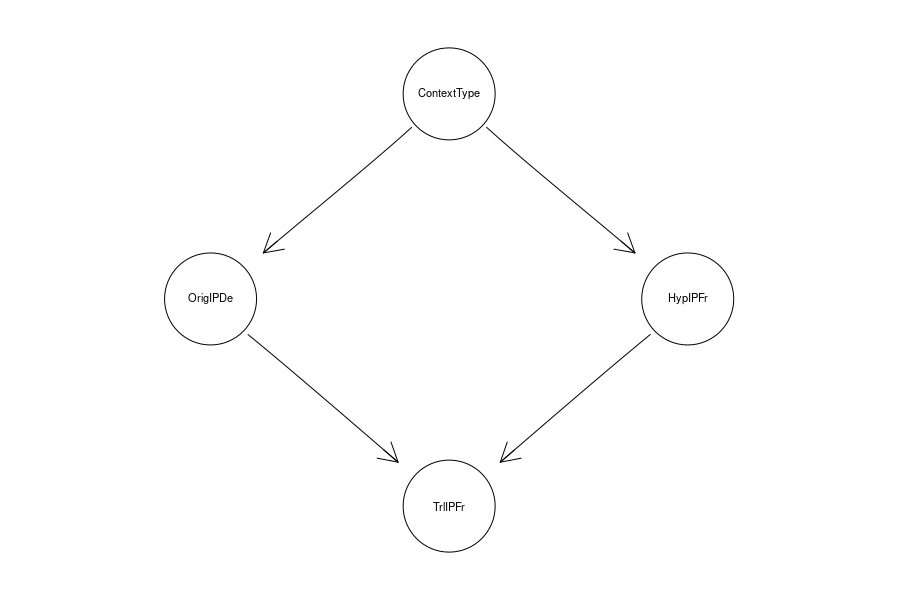
\includegraphics[width=0.9\linewidth]{figures/bilingual-model.jpeg}}
   \put(100,410){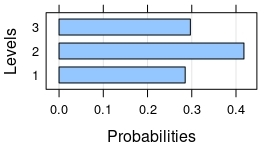
\includegraphics[width=0.3\linewidth]{figures/ProbsContextType.jpeg}}
   \put(0,340){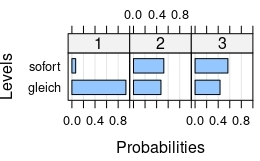
\includegraphics[width=0.3\linewidth]{figures/CondProbsOrigIPDe.jpeg}}
   \put(215,340){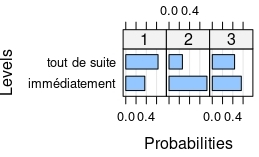
\includegraphics[width=0.3\linewidth]{figures/CondProbsHypIPFr.jpeg}}
   \put(30,110){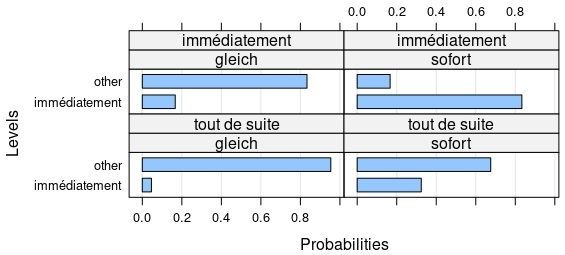
\includegraphics[width=0.6\linewidth]{figures/CondProbsTrlIPFr.jpeg}}
 \end{picture}
 %\end{minipage}
  \cprotect\caption{Directed acyclic graph for IP-adverbials
     (comparative/directional, with clustered observations). The graph
     was created with the package \verb+bnlearn+ for \verb+R+ \citep{bnlearn-package}.}
   \label{fig:BilingualModel}
\end{figure}


%\begin{itemize}
%\item
  The distribution of \textbf{Context types} is represented at the top of
  the graph. We assume the three types distinguished by the
  `smaller' PAM-cluster solution
  (cf. Sect. \ref{sec:ComparativeUndirected}). Each of the context
  types has a certain (relative) frequency. 
We estimated the frequencies of the three context types from our sample.

% \item
The specific context type conditions a frequency distribution in the
originals. We can, again, determine this distribution on the basis of
our sample. The node \textbf{OrigIPDe} is associated with conditional
probabilities of the form $p(w_{de}|c)$ -- the probability of using
a specific German \ipadv $w_{de}$, given a context $c$.

% \item
The node \textbf{HypIpFr} stands for a hypothetically used French \ipadv\ --
the \ipadv\ that \textit{may} have been used in monolingual (French) language
production, in the specific context. Like the node OrigIPDe, this
node is associated with a conditional frequency distribution,
$p(w_{fr}|c)$. This distribution can be estimated from the original
French data.

% \item
Finally, the node \textbf{TrlIPFr} stands for the \ipadv\ used in the French
translation from German. According to the DAG in Figure
\ref{fig:BilingualModel}, this choice is conditioned by the
probability of using a specific French expression (as in monolingual
language production), and the influence from the German \ipadv,
reflecting form-to-form associations in translation. 
The node TrlIPFr thus represents a distribution over French \ipadv s,
conditioned by the hypothetical French \ipadv\ and the German \ipadv\
in the original sentence. % In order to define this distribution, we
% infered the use of a French IP-adverbial based on the associations
% between context types and original French data.
This distribution cannot be observed, as no (hypothetical) monolingual
\ipadv\ is ever produced in French translation from German. In order
to infer the hypothetical French expressions, we trained a classifier
(a support vector machine/SVM) on all explanatory variables, predicting a
given \ipadv\ for each translated French sentence.\footnote{The
  model has an accuracy of 88.2\% for the entire training set, and of
  79.5\% with a 0.9/0.1 training/test split, averaging over ten-fold
  cross-validation. We used a radial kernel, with $C=3$ and
  $\gamma=0.1$.}
%\end{itemize}

The network shown in Figure \ref{fig:BilingualModel} represents a
hypothesis about mediated language production.  By breaking down the
joint probability distribution into local, partially independent
distributions, we can model components of the highly complex process
of mediated language production.
%
As our data set is quite small and the estimates for some parameters
are not very precise, we will illustrate this procedure with a binary
choice, by modeling the use of \textit{immédiatement} in French
translations. All French \ipadv s other than \textit{immédiatement}
were subsumed under the category of `other'.

The Bayesian network in Figure \ref{fig:BilingualModel} allows us to
determine theoretical distributions of French \ipadv s under
different conditions, and to compare them to the empirical
distributions. This can give us an estimate of the plausibility of the
causal model.
%
Tables \ref{tab:ProbTab} shows the empirical probabilities on the left
and the theoretical probabilities (according to the Bayesian network)
on the right. While the ranks of the expressions -- by context type
and \ipadv\ -- are identical, the two distributions are considerably
different. Even though the model in the form displayed in Figure
\ref{fig:BilingualModel} may not be entirely realistic, it provides
a starting point for a more elaborate model. This
is one of the main assets of Bayesian networks: they can be extended
and built up step by step, and their graphical nature helps
researchers to develop an understanding of the data.

\begin{table}[t]
  \begin{tabular}{l|ll|ll}
            & \multicolumn{2}{c|}{empirical} & \multicolumn{2}{c}{theoretical}\\\cline{2-5}    
ContextType &  \textit{gleich}     &   \textit{sofort}  & \textit{gleich} & \textit{sofort} \\\hline
1           & 0    & 0.25 & 0.09     & 0.51\\
2           & 0.24 & 0.53 & 0.13      & 0.7\\
3           & 0.07 & 0.48 & 0.11      & 0.61\\
  \end{tabular}
  \cprotect\caption{Empirical probabilities (left) and theoretical probabilities
    according to the Bayesian network (right) for the occurrence of
    \textit{immédiatement} in French translations, in specific
    contexts, given a specific German \ipadv\ in the original.}
  \label{tab:ProbTab}
\end{table}


%%% Local Variables:
%%% mode: latex
%%% TeX-master: "main"
%%% End:
